\documentclass[letterpaper,12pt]{article}
\usepackage{fullpage}
\usepackage{amsmath}
\usepackage{graphicx}
\usepackage{epsfig}

% This last command gives the possibility of variable line spacing.
\renewcommand{\baselinestretch}{1.1}
\newcommand{\bqu}{\begin{quote} \it}
\newcommand{\equ}{\end{quote}}
\newcommand{\beqn}{\begin{eqnarray}}
\newcommand{\eeqn}{\end{eqnarray}}
\newcommand{\nonu}{\nonumber \\}
\newcommand{\br}{\langle}
\newcommand{\ke}{\rangle}
\def\f#1#2{\frac{#1}{#2}}

\def\ni{\noindent}
\def\J{{\rm\,J}}
\def\W{{\rm\,W}}
\def\s{{\rm\,s}}
\def\erg{{\rm\,erg}}
\def\cm{{\rm\,cm}}
\def\m{{\rm\,m}}
\def\km{{\rm\,km}}
\def\kg{{\rm\,kg}}
\def\mm{{\rm\,mm}}
\def\gm{{\rm\,g}}
\def\g{{\rm\,g}}
\def\d{\rm\,d}
\def\h{\rm\,h}
\def\mum{\,\mu{\rm m}}
\def\K{{\rm\,K}}
\def\yr{{\rm\,yr}}
\def\Hz{{\rm\,Hz}}
\def\days{{\rm\,days}}
\def\cals{{\rm\,cals}}
\def\mole{{\rm\,mole}}
\def\gal{{\rm\,gal}}
\def\calo{\,{\rm calorie}}
\def\dyne{\,{\rm dyne}}
\def\s{\,{\rm s}}
\def\at{\, {\rm atmosphere}}
\def\J{\,{\rm joule}}
\def\pomega{\tilde{\omega}}
\def\vs{\vspace{0.1in}}
\def\n{\vspace{0.1in} \ni }

\begin{document}

Max Genecov

\begin{center}
\Large Stellar Populations Homework 3, Question 2
\end{center}

\normalsize


\section{Fitting Integrated Light}

Once again, python-fsps has failed me on jupyter notebooks, (any way to work around this?) so here are my plots are cumulated thoughts. My python instructions are in the HW3P2.py file with a bit of the repetition cut out.

I was not sure how to include stellar evolution and atmosphere models in fsps, so I used the defaults. The IMF is also the default Kroupa IMF. Also, the definition of zmet allows a choice of only -2.5 and -2.0 when I would prefer something in the middle. Also, zmet only takes integer values, a rounding complicates our distributions a bit. I chose zmet = 1.

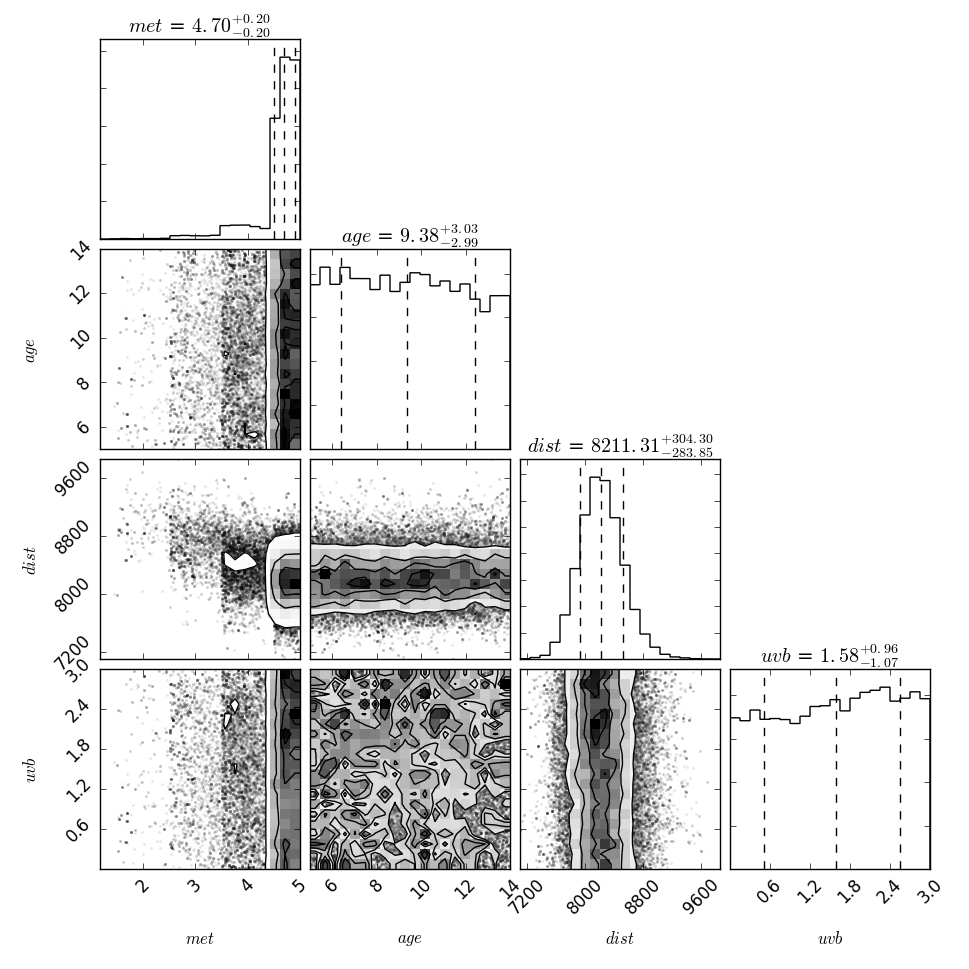
\includegraphics[width=5.5in]{corner1}

There is no apparent constraint for the age or the extinction. The distributions appear uniform within the flat priors. With this, there comes an incorrect assessment of the metallicity (originally 1). If I make a harsher prior in the age, I get a longer tail for the metallicity, but the mean value is still above 4, and the age and extinction are still uniform.

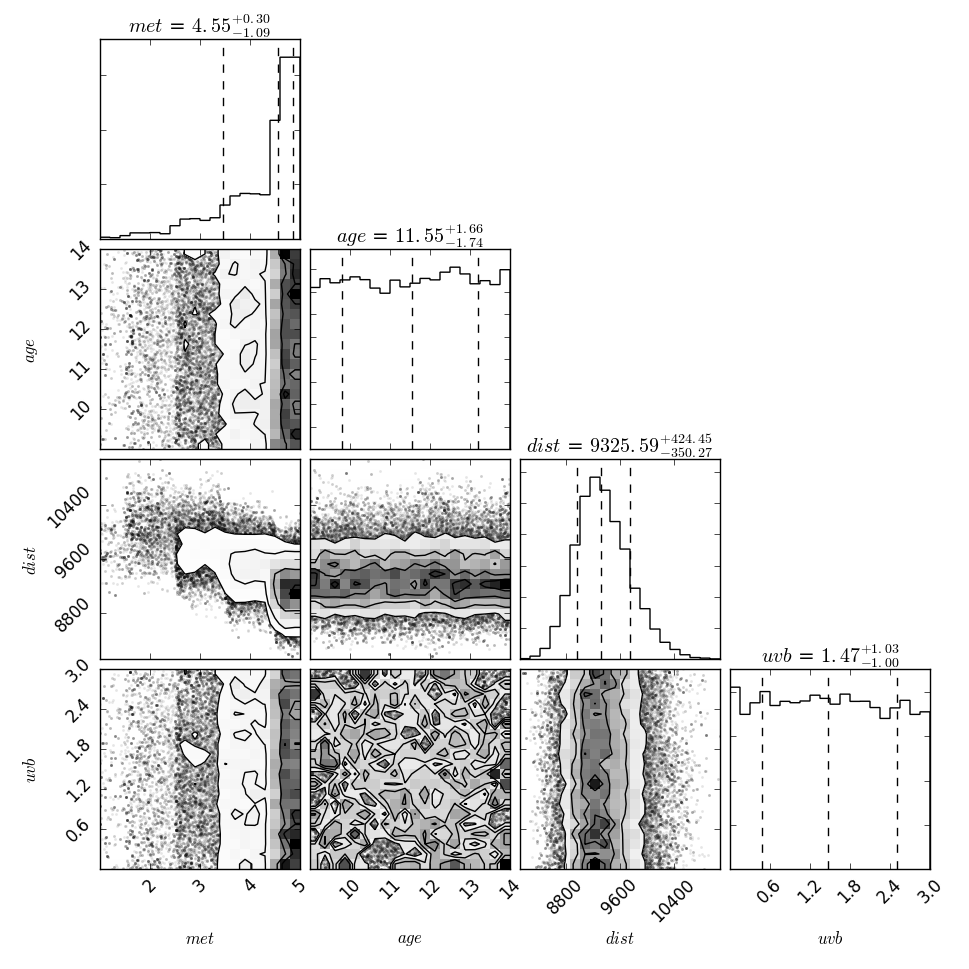
\includegraphics[width=5.5in]{corner11}

When I reduce the uncertainties from .1 mag to .01 mag, it takes emcee longer to reach an equilibrium, but the corner plots are more interesting. 

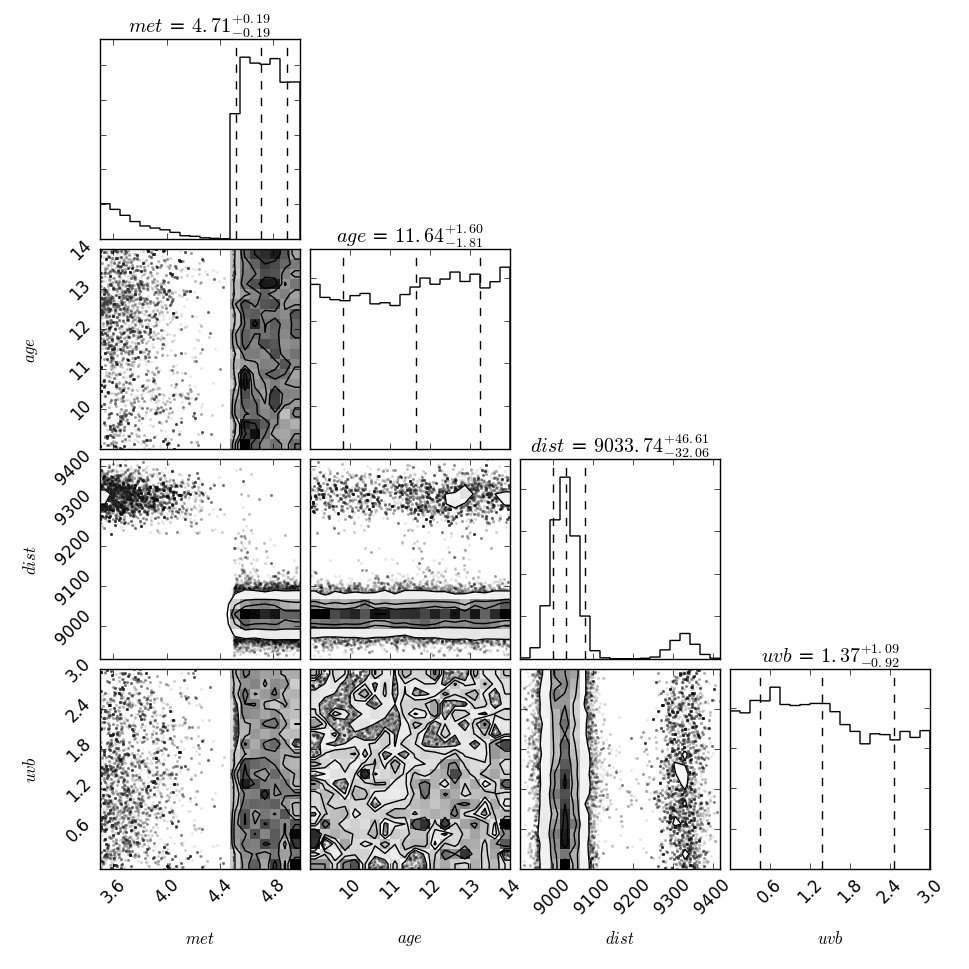
\includegraphics[width=5.5in]{corner21}

There are now two peaks in both the metallicity and the distance, though the new one is much smaller than the other. The distance is now a little more like the input value, but the metallicity peaks are still too high compared to the initial.

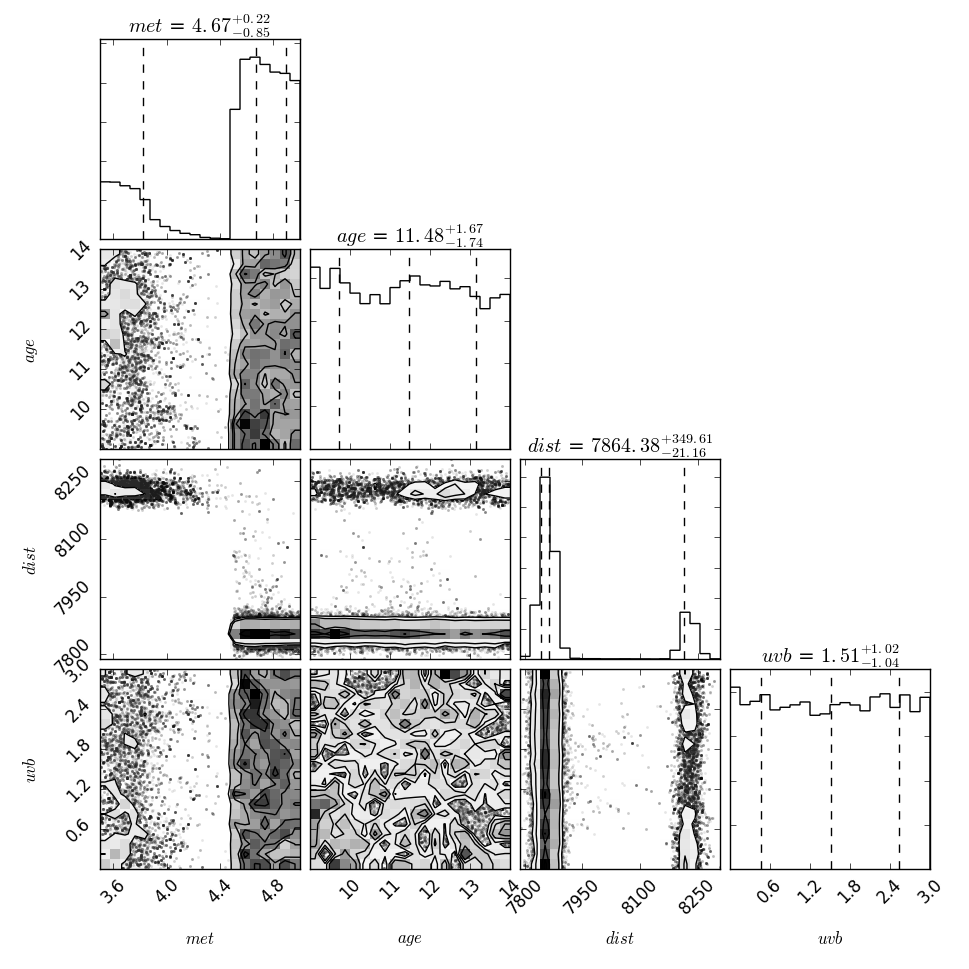
\includegraphics[width=5.5in]{corner31}

Things don't get much better when we include the other two filters with errors of .01 mag. The metallicity isn't much different, though the secondary peak at zmet = 3 is now higher. There is now a peak at basically the same location as the input now. In the higher uncertainty version of this plot (.1 mag), there appeared to be a linear relationship between zmet and distance at lower values. That is not the case now; the secondary peaks do correspond to lower metallicity and higher distance, but it is no longer a continuous correlation. Still the age and extinction are functionally free parameters. 

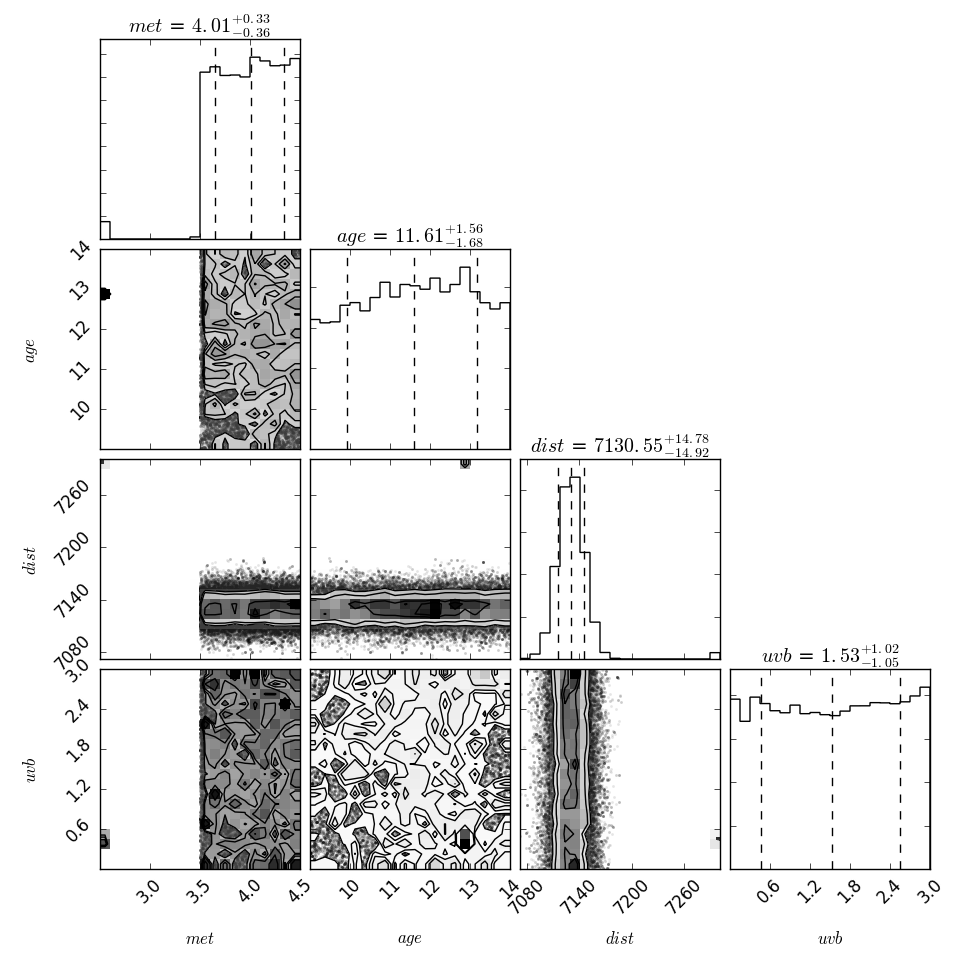
\includegraphics[width=5.5in]{corner41}

Including the FUV doesn't help our case at all! In fact, we now have worse parameters than we did with the four filters. It is initially unclear to me as to why more data might provide a worse fit. Perhaps it is because the UV magnitudes are produced in a different way than they are solved for, but I have no idea why that would be or what those methods might entail. It is now very late and I will try to dream up some physical basis for this while I sleep, but it will probably be drowned out by another teeth-falling-out nightmare.

\end{document}